\newpage
\section{Durchführung}
    \subsection{Versuchsaufbau}
        Um die Spektrallinien und deren Aufspaltung zu vermessen, wird eine Cadmium-Spektrallampe innerhalb eines Elektromagnetens so platziert, dass das Licht der Lampe senkrecht zu den Magnetfeldlinien 
        beobachtet werden kann. Dieses ausgesendete Licht wird zunächst durch das Objetiv O kollimiert und anschließend durch die Kondensorlinse L$_1$ möglichst genau auf den Spalt S$_1$ abgebildet. Hinter 
        dem Spalt wird das Licht durch die Linse L$_2$ erneut kollimiert und durchläuft daraufhin ein Geradsichtprisma, in dem die Wellenlängenkomponenten aufgrund unterschiedlich starker Brechung räumlich 
        getrennt werden. Es ergeben sich eine grüne, blaue, dunkelblaue und rote Komponente. Die nun getrennten Komponenten durchlaufen einen Polarisationsfilter, der ermöglicht nur ausgewählte Übergänge zu 
        beobachten und werden durch die Linse L$_3$ auf einen weiteren Spalt S$_2$ fokussiert. Dieser ist verschiebbar, sodass eine ausgewählte Wellenlängenkomponenten den Spalt durchlaufen kann, während alle 
        anderen Komponenten blockiert werden. Zuletzt wird das Licht über die Linse L$_4$ auf die Lummer-Gehrcke-Platte fokussiert. Diese ist in Abbildung \ref{fig:lummer} dargestellt und erzeugt ein 
        Interferenzmuster, wenn die Bragg-Bedingung

        \begin{equation*}
            2nd\cos(\beta) = m\lambda,
        \end{equation*}

        wobei $d$ die Dicke der Platte, $\lambda$ die Wellenlänge des Lichts, $n$ der Brechungsindex des Glases, $\beta$ der Reflexionswinkel innerhalb der Platte und $m$ die Ordnung des Interferenzmaximas ist.
        Das Interferenzbild wird über eine Digitalkamera aufgenommen und ermöglicht die Bestimmung der Wellenlänge des Lichts.
        \subsubsection*{Auflösungsvermögen und Dispersionsgebiet der Lummer-Gehrcke-Platte}
            Eine Veränderung des Magnetfeldes hat eine Wellenlängenverschiebung
            \begin{equation}
                \delta\lambda=\frac{1}{2}\frac{\delta s}{\Delta s}\Delta\lambda_D
            \end{equation}
            zur Folge. $\Delta s$ ist dabei der Linienabstand bei abgeschaltetem Magnetfeld und
            $\delta s$ die Verschiebung der Linien wenn das Feld angeschaltet wird.
            \begin{equation}
                \Delta\lambda_D=\frac{\lambda^2}{2d}\sqrt{\frac{1}{n^2-1}}
                \label{eqn:delta_lambda}
            \end{equation}
            ist das sogennante Dispersionsgebiet, welches die nötige Differenz angibt,
            sodass sich zwei Wellenlängen nicht überlagern. Für eine gegebene Wellenlänge $\lambda$ lässt sich das Auflösungsvermögen der Lummer-Gehrcke-Platte über folgende Formel
            
            \begin{equation}
                A = \frac{L}{\lambda} (n^2 - 1),
                \label{eqn:auflösung}
            \end{equation}

            die die Länge der Lummer-Gehrcke-Platte $L$ und den Brechungsindex des Materials der Platte $n$ enthält.

            So lassen sich für die zu untersuchenden Übergänge folgende Dispersionsgebiete und Auflösungsvermögen berechnen:
            
            \begin{align*}
                \Delta\lambda_{D, \SI{643.8}{\nano\metre}} = \SI{48.91}{\pico\metre}  \qquad A_{\SI{643.8}{\nano\metre}} = \num{2.09e5} \\
                \Delta\lambda_{D, \SI{480.0}{\nano\metre}} = \SI{26.95}{\pico\metre}  \qquad A_{\SI{480.0}{\nano\metre}} = \num{2.85e5}
            \end{align*}




        \begin{figure}[h]
            \centering
            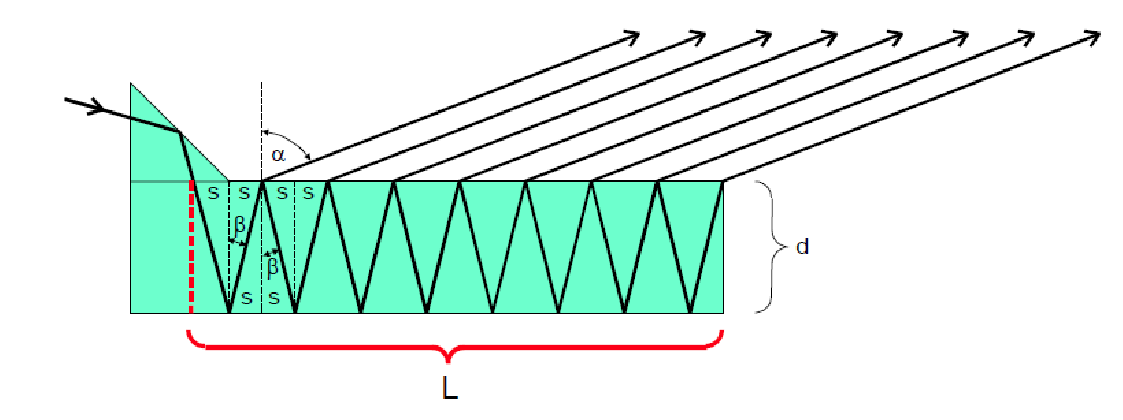
\includegraphics[width = 0.9\textwidth]{pictures/lummer.png}
            \caption{Schematischer Aufbau der Lummer-Gehrcke Platte, deren erzeugtes Interferenzmuster zur Bestimmung der Wellenlängenverschiebung genutzt wird. Entnommen aus \cite{tu_dortmund_versuchsanleitung_2021-5}}
            \label{fig:lummer}
        \end{figure}

        \FloatBarrier

        \begin{figure}[h]
          \centering
          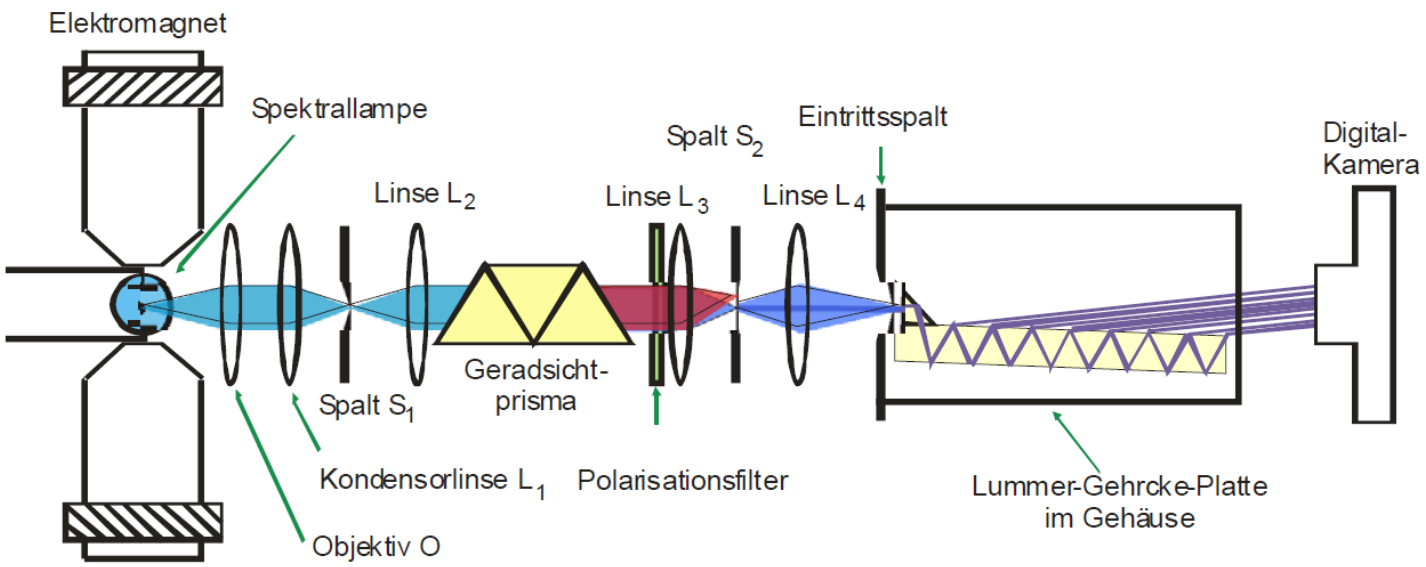
\includegraphics[width = 0.8\textwidth]{pictures/Aufbau.png}
          \caption{Der Aufbau zur Vermessung der Spektrallinien sowie deren Aufspaltung. Das Licht stammt aus einer Cadmium-Spektrallampe und die Spektrallinien werden durch einen Elektromagneten aufgespalten. Anschließend wird das Licht durch ein Geradsichtprisma räumlich in seine Wellenlängenkomponenten zerlegt. Die Komponenten können einzeln auf eine Lummer-Gehrcke-Platte abgebildet werden und erzeugen dort ein Interferenzbild. Entnommen aus \cite{tu_dortmund_versuchsanleitung_2021-5}}
          \label{fig:Aufbau}
        \end{figure}
    
        \FloatBarrier

    

    \subsection{Kalibrierung des Magnetfelds}
        Für die Auswertung der Aufspaltung ist die Kenntnis des angelegten Magnetfelds notwendigs. Da das Magnetfeld jedoch nicht gemessen werden kann, während die Spektrallampe in den Elektromagneten 
        eingesetzt ist, wird das Magnetfeld im Zentrum des Elektromagneten zunächst kalibriert. Dazu wird das Magnetfeld in Abhängigkeit vom angelegtem Spulenstrom mit einer Hall-Sonde im Bereich von 
        \SI{0.4}{\ampere} bis \SI{7.2}{\ampere} vermessen. So soll ein Zusammenhang zwischen Magnetfeldstärke und Stromstärke ermittelt werden, der es ermöglicht die angelegte Magnetfeldstärke über den 
        Spulenstrom zu berechnen.   

    \subsection{Vermessung der Spektrallinienaufspaltung}
        \subsubsection*{Vermessung des normalen Zeeman-Effekts}
            Zur Vermessung des normalen Zeeman-Effekts wird die rote Spektrallinie untersucht. Dazu wird diese auf die Lummer-Gehrcke-Platte abgebildet und das Interferenzbild für vier Fälle aufgenommen.
            
            \begin{enumerate}
                \item I$_{\text{Spule}}$ = \SI{0}{\ampere}, $\qquad$    $\varphi_{\text{Pol}}$ = \SI{0}{\degree}
                \item I$_{\text{Spule}}$ = \SI{0}{\ampere}, $\qquad$    $\varphi_{\text{Pol}}$ = \SI{90}{\degree}
                \item I$_{\text{Spule}}$ = \SI{5}{\ampere}, $\qquad$    $\varphi_{\text{Pol}}$ = \SI{0}{\degree}
                \item I$_{\text{Spule}}$ = \SI{5}{\ampere}, $\qquad$    $\varphi_{\text{Pol}}$ = \SI{90}{\degree}
            \end{enumerate}

            In den ersten beiden Fällen liegt kein Magnetfeld an und die Spektrallinie sollte nicht aufgespalten sein. Im dritten und vierten Fall sind die Spektrallinien aufgespalten. Es sollte dennoch nur 
            im dritten Fall eine optische Aufspaltung erkennbar sein, da das Licht des normalen Übergangs hier nicht durch den Polarisationsfilter herausgefiltert wird.
            
            
        \subsubsection*{Vermessung des anormalen Zeeman-Effekts}
            Zur Vermessung des anormalen Zeeman-Effekts wird die blaue Spektrallinie untersucht. Diese wird wie die rote auf die Lummer-Gehrcke-Platte abgebildet und das Interferenzbild für folgende vier Fälle 
            aufgenommen. Hier ist der letzte Fall durch eine Magnetfeldstärke definiert, da die zugehörigen Daten aus einem externen Experiment übernommen werden mussten.
            
            \begin{enumerate}
                \item I$_{\text{Spule}}$ = \SI{0}{\ampere}, $\qquad$    $\varphi_{\text{Pol}}$ = \SI{0}{\degree}
                \item I$_{\text{Spule}}$ = \SI{0}{\ampere}, $\qquad$    $\varphi_{\text{Pol}}$ = \SI{90}{\degree}
                \item I$_{\text{Spule}}$ = \SI{2.6}{\ampere}, $\qquad$    $\varphi_{\text{Pol}}$ = \SI{0}{\degree}
                \item B$_{\text{Spule}}$ = \SI{1.009}{\tesla}, $\qquad$    $\varphi_{\text{Pol}}$ = \SI{90}{\degree}
            \end{enumerate}

            Erneut sollte für die ersten beiden Fällen keine Aufspaltung zu sehen sein. Im dritten und vierten Fall sind die Spektrallinien erneut aufgespalten. Bei dieser Beobachtung sollte die optische 
            Aufspaltung im Gegensatz zur Beobachtung des normalen Zeeman-Effekts im vierten Fall bei einem Polarisationswinkel von \SI{90}{\degree} zu sehen sein.
        
